\documentclass[11pt]{article}
% ===========================================================================
%  Shared preamble for all MPM2D worksheets — input right after \documentclass.
%  (Files beginning with "_" are skipped by mpm2d-worksheet-publish.mjs.)
% ===========================================================================
\usepackage[letterpaper,top=2.2cm,bottom=1.9cm,left=1.6cm,right=1.6cm,headheight=28pt,footskip=24pt]{geometry}
\usepackage{amsmath,amssymb}
\usepackage{cancel}
\usepackage[T1]{fontenc}
\usepackage[utf8]{inputenc}
\usepackage{lmodern}
\usepackage{xcolor}
\usepackage[most]{tcolorbox}
\usepackage{enumitem}
\usepackage{multicol}
\usepackage{fancyhdr}
\usepackage{tikz}
\usetikzlibrary{calc}
\usepackage{pgfplots}
\pgfplotsset{compat=1.18}

\definecolor{exblue}{HTML}{4A90E2}
\definecolor{exbg}{HTML}{E6F3FF}
\definecolor{qorange}{HTML}{E69138}
\definecolor{qbg}{HTML}{FFF7CC}
\definecolor{keygray}{HTML}{475569}
\definecolor{keybg}{HTML}{F1F5F9}
\definecolor{iagreen}{HTML}{14653B}
\definecolor{titleblue}{HTML}{1D4ED8}
% Rotating palette so each worked example gets its own colour.
\definecolor{ex0}{HTML}{2563A0}\definecolor{ex1}{HTML}{3B7D3B}\definecolor{ex2}{HTML}{8A5A00}
\definecolor{ex3}{HTML}{A3327A}\definecolor{ex4}{HTML}{6D28A3}\definecolor{ex5}{HTML}{B08900}
\definecolor{ex6}{HTML}{0E7490}\definecolor{ex7}{HTML}{9A3412}\definecolor{ex8}{HTML}{15803D}

\pagestyle{fancy}
\fancyhf{}
\fancyhead[L]{\footnotesize NAME: \underline{\hspace{3.4cm}}}
\fancyhead[C]{\textbf{Integration Academy}\\[-2pt]{\scriptsize Math Simplified \textperiodcentered{} Success Amplified}}
\fancyhead[R]{\footnotesize MPM2D}
\fancyfoot[L]{\scriptsize dr.merie@IntegrationAcademy.ca}
\fancyfoot[C]{\scriptsize\thepage}
\fancyfoot[R]{\scriptsize IntegrationAcademy.ca}
\renewcommand{\headrulewidth}{1.2pt}
\renewcommand{\footrulewidth}{0.4pt}
\setlength{\parindent}{0pt}
\setlength{\parskip}{4pt}

% Examples are NOT breakable, so each example + its solution stays on one page.
\newtcolorbox{example}[2]{colframe=#1,colback=#1!7,coltitle=white,colbacktitle=#1,fonttitle=\bfseries,title={#2},arc=3pt,boxrule=1pt}
\newtcolorbox{qbox}[1]{colframe=qorange,colback=qbg,coltitle=white,colbacktitle=qorange,fonttitle=\bfseries,title={#1},arc=3pt,breakable,boxrule=1pt}
\newtcolorbox{keybox}{colframe=keygray,colback=keybg,coltitle=white,colbacktitle=keygray,fonttitle=\bfseries,title={$\checkmark$\ Answer Key},arc=3pt,breakable,boxrule=1pt}
\newtcolorbox{recapbox}{colframe=keygray,colback=keybg,coltitle=white,colbacktitle=keygray,fonttitle=\bfseries,title={Question Recap},arc=3pt,breakable,boxrule=1pt}
\newtcolorbox{ideabox}{colframe=titleblue,colback=titleblue!6,coltitle=white,colbacktitle=titleblue,fonttitle=\bfseries,title={The Big Ideas},arc=3pt,breakable,boxrule=1.2pt}
\newtcolorbox{learnbox}{colframe=iagreen,colback=iagreen!5,coltitle=white,colbacktitle=iagreen,fonttitle=\bfseries,title={The Big Picture},arc=3pt,breakable,boxrule=1.2pt}
\newcommand{\lh}[1]{\par\smallskip{\bfseries\color{iagreen}#1}\par\nobreak\smallskip}

\newcommand{\soln}{\par\smallskip\textit{\textbf{Solution.}}\ }
\newcommand{\workspace}[1]{\par\vspace{3pt}\fcolorbox{black!30}{white}{\begin{minipage}[t][#1][t]{\dimexpr\linewidth-2\fboxsep\relax}\ \end{minipage}}\par}
\newcommand{\sech}[1]{\par\vspace{8pt}{\Large\bfseries\color{iagreen}#1}\par\nobreak\vspace{2pt}{\color{black!20}\hrule height1pt}\vspace{6pt}}

% A compact coordinate plot sized for an example box: \eplot{xmin}{xmax}{ymin}{ymax}{body}
\newcommand{\eplot}[5]{\begin{center}\begin{tikzpicture}
\begin{axis}[width=6.8cm,height=4.4cm,axis lines=middle,xlabel={\tiny$x$},ylabel={\tiny$y$},
grid=both,grid style={gray!16},xmin=#1,xmax=#2,ymin=#3,ymax=#4,
xtick distance=2,ytick distance=2,tick label style={font=\tiny},axis line style={-},samples=120]
#5
\end{axis}\end{tikzpicture}\end{center}}

% A sine-curve plot (degrees on x, 0..360): \splot{ymin}{ymax}{body}
\newcommand{\splot}[3]{\begin{center}\begin{tikzpicture}
\begin{axis}[width=8.6cm,height=4.6cm,axis lines=middle,xlabel={\tiny$x\,(^\circ)$},ylabel={\tiny$y$},
grid=both,grid style={gray!16},xmin=0,xmax=360,ymin=#1,ymax=#2,
xtick distance=90,ytick distance=1,tick label style={font=\tiny},axis line style={-},samples=180]
#3
\end{axis}\end{tikzpicture}\end{center}}

% A small coordinate plot: \plot{xmin}{xmax}{ymin}{ymax}{body}
\newcommand{\plot}[5]{\begin{center}\begin{tikzpicture}
\begin{axis}[width=8.4cm,height=6cm,axis lines=middle,xlabel={\scriptsize$x$},ylabel={\scriptsize$y$},
grid=both,grid style={gray!16},xmin=#1,xmax=#2,ymin=#3,ymax=#4,
xtick distance=2,ytick distance=2,tick label style={font=\tiny},axis line style={-}]
#5
\end{axis}\end{tikzpicture}\end{center}}

% Right triangle (angle theta at bottom-left, right angle at bottom-right):
%   \rtri{drawBase}{drawHeight}{oppLabel}{adjLabel}{hypLabel}
\newcommand{\rtri}[5]{\begin{center}\begin{tikzpicture}[scale=0.85]
\coordinate (A) at (0,0);\coordinate (B) at (#1,0);\coordinate (C) at (#1,#2);
\draw[thick,exblue] (A)--(B)--(C)--cycle;
\draw[black] ($(B)+(-0.32,0)$)--($(B)+(-0.32,0.32)$)--($(B)+(0,0.32)$);
\node[below] at ($(A)!0.5!(B)$){#4};
\node[right] at ($(B)!0.5!(C)$){#3};
\node[above left] at ($(A)!0.5!(C)$){#5};
\node at (0.7,0.22){$\theta$};
\end{tikzpicture}\end{center}}

% General (oblique) triangle with vertex labels and opposite-side labels:
%   \gtri{Alabel}{Blabel}{Clabel}{aSide}{bSide}{cSide}
\newcommand{\gtri}[6]{\begin{center}\begin{tikzpicture}[scale=0.85]
\coordinate (A) at (0,0);\coordinate (B) at (5,0);\coordinate (C) at (1.6,3);
\draw[thick,exblue] (A)--(B)--(C)--cycle;
\node[below left] at (A){#1};\node[below right] at (B){#2};\node[above] at (C){#3};
\node[below] at ($(A)!0.5!(B)$){#6};
\node[right] at ($(B)!0.5!(C)$){#4};
\node[left] at ($(A)!0.5!(C)$){#5};
\end{tikzpicture}\end{center}}

\fancyhead[R]{\footnotesize MCV4U \textperiodcentered{} 6.2}
\begin{document}

\begin{center}
{\LARGE\bfseries\color{titleblue}Worksheet 6.2 --- Vector Operations (Geometric)}\\[2pt]
{\small Grade 12 Calculus and Vectors (MCV4U) \textperiodcentered{} Unit 6: Geometry and Algebra of Vectors}
\end{center}

\begin{ideabox}
Add tip-to-tail (triangle law); subtract via $\vec a-\vec b=\vec a+(-\vec b)$; scale by $k$ to change length (and flip if $k<0$).
\begin{itemize}[leftmargin=*,itemsep=2pt]
  \item Addition: tip-to-tail; resultant from first tail to last tip.
  \item Subtraction: $\vec a-\vec b=\vec a+(-\vec b)$.
  \item $k\vec v$ has length $|k||\vec v|$; reversed if $k<0$.
\end{itemize}
\end{ideabox}

\begin{learnbox}
\lh{Adding vectors}Add vectors \textbf{tip-to-tail}: the resultant runs from the first tail to the last tip. The parallelogram rule gives the same result.
\lh{Scalar multiples}Multiplying by a scalar scales the length and, if negative, reverses the direction while keeping the line of action.
\lh{Subtraction}Subtracting a vector means adding its opposite, which the triangle of vectors makes easy to picture.
\end{learnbox}

\sech{Worked Examples}

\begin{example}{ex0}{Example 1 --- Perpendicular resultant}
Add 3 east and 4 north; find the resultant.\soln
\textbf{Step 1 (the two vectors are perpendicular, so use the Pythagorean theorem for magnitude):} $|\vec R|=\sqrt{3^2+4^2}=\sqrt{9+16}=\sqrt{25}$.\\[3pt]
\textbf{Step 2 (find the direction with $\tan^{-1}$ of opposite over adjacent):} $\theta=\tan^{-1}\tfrac43\approx53^\circ$ north of east.\\[3pt]
\textbf{Conclusion:} magnitude $5$, direction $\approx53^\circ$ N of E:\begin{center}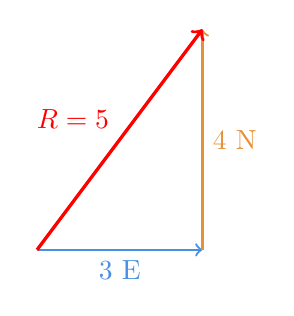
\begin{tikzpicture}[scale=0.7]\draw[->,thick,exblue](0,0)--(3,0)node[midway,below]{$3$ E};\draw[->,thick,qorange](3,0)--(3,4)node[midway,right]{$4$ N};\draw[->,very thick,red](0,0)--(3,4)node[midway,above left]{$R=5$};\end{tikzpicture}\end{center}
\end{example}

\begin{example}{ex1}{Example 2 --- Triangle law}
How do you draw $\vec a+\vec b$?\soln
\textbf{Step 1 (draw $\vec a$ first):} start anywhere and draw $\vec a$.\\[3pt]
\textbf{Step 2 (attach $\vec b$ tip-to-tail):} place the tail of $\vec b$ at the tip (arrowhead) of $\vec a$.\\[3pt]
\textbf{Step 3 (draw the resultant):} the sum $\vec a+\vec b$ runs from $\vec a$'s starting tail to $\vec b$'s final tip.\\[3pt]
\textbf{Conclusion:} tip-to-tail, then close the triangle from the first tail to the last tip.
\end{example}

\begin{example}{ex2}{Example 3 --- Scalar multiple}
Describe $3\vec v$ and $-2\vec v$.\soln
\textbf{Step 1 (scalar multiplication scales the length by $|k|$):} for $3\vec v$, $|k|=3$; for $-2\vec v$, $|k|=2$.\\[3pt]
\textbf{Step 2 (the sign of $k$ determines direction):} positive $k$ keeps the same direction; negative $k$ reverses it.\\[3pt]
\textbf{Conclusion:} $3\vec v$ is three times as long, same direction; $-2\vec v$ is twice as long, opposite direction.
\end{example}

\begin{example}{ex3}{Example 4 --- Subtraction}
How do you draw $\vec a-\vec b$?\soln
\textbf{Step 1 (rewrite subtraction as addition of the opposite):} $\vec a-\vec b=\vec a+(-\vec b)$.\\[3pt]
\textbf{Step 2 (draw $-\vec b$, i.e.\ $\vec b$ reversed):} flip $\vec b$'s direction, keeping its length.\\[3pt]
\textbf{Step 3 (add tip-to-tail):} attach $-\vec b$'s tail to $\vec a$'s tip, as in ordinary addition.\\[3pt]
\textbf{Conclusion:} draw $\vec a$, then add the reversed $\vec b$ tip-to-tail.
\end{example}

\begin{example}{ex4}{Example 5 --- Resultant force}
Forces 6 N east and 8 N north. Find the resultant.\soln
\textbf{Step 1 (perpendicular components, use Pythagorean theorem):} $|\vec R|=\sqrt{6^2+8^2}=\sqrt{36+64}=\sqrt{100}$.\\[3pt]
\textbf{Step 2 (find the direction):} $\theta=\tan^{-1}\tfrac86\approx53^\circ$ north of east.\\[3pt]
\textbf{Conclusion:} $10$ N at $\approx53^\circ$ N of E.
\end{example}

\begin{example}{ex5}{Example 6 --- Perpendicular resultant}
Resultant magnitude of 5 east and 12 north?\soln
\textbf{Step 1 (Pythagorean theorem, since the components are perpendicular):} $\sqrt{5^2+12^2}=\sqrt{25+144}=\sqrt{169}$.\\[3pt]
\textbf{Conclusion:} $13$.
\end{example}

\begin{example}{ex6}{Example 7 --- Scalar multiple}
Describe $-\tfrac12\vec v$.\soln
\textbf{Step 1 (magnitude scales by $|k|=\tfrac12$):} half the original length.\\[3pt]
\textbf{Step 2 (negative $k$ reverses direction):} points opposite to $\vec v$.\\[3pt]
\textbf{Conclusion:} half the length, opposite direction.
\end{example}

\begin{example}{ex7}{Example 8 --- Perpendicular resultant}
Resultant magnitude of 9 east and 12 north?\soln
\textbf{Step 1 (Pythagorean theorem):} $\sqrt{9^2+12^2}=\sqrt{81+144}=\sqrt{225}$.\\[3pt]
\textbf{Conclusion:} $15$.
\end{example}

\begin{example}{ex8}{Example 9 --- Direction}
Direction of the resultant of 3 east, 4 north?\soln
\textbf{Step 1 (set up the tangent ratio, opposite over adjacent):} $\tan\theta=\tfrac{4}{3}$ (north component over east component).\\[3pt]
\textbf{Step 2 (solve for $\theta$):} $\theta=\tan^{-1}\tfrac43\approx53^\circ$.\\[3pt]
\textbf{Conclusion:} $\approx53^\circ$ north of east.
\end{example}

\clearpage
\sech{Your Turn --- Show Your Work}
For each question, show all steps clearly in the space provided.

\begin{qbox}{Question 1}
Resultant magnitude of 5 east and 12 north?\workspace{2.4cm}
\end{qbox}

\begin{qbox}{Question 2}
Describe $4\vec v$.\workspace{2.4cm}
\end{qbox}

\begin{qbox}{Question 3}
Describe $-\tfrac13\vec v$.\workspace{2.4cm}
\end{qbox}

\begin{qbox}{Question 4}
Resultant magnitude of 8 east and 15 north?\workspace{2.4cm}
\end{qbox}

\begin{qbox}{Question 5}
What law adds vectors tip-to-tail?\workspace{2.4cm}
\end{qbox}

\begin{qbox}{Question 6}
Resultant magnitude of 6 east and 8 north?\workspace{2.4cm}
\end{qbox}

\begin{qbox}{Question 7}
Describe $-3\vec v$.\workspace{2.4cm}
\end{qbox}

\begin{qbox}{Question 8}
Resultant magnitude of 7 east and 24 north?\workspace{2.4cm}
\end{qbox}

\begin{qbox}{Question 9}
How do you express $\vec a-\vec b$ as an addition?\workspace{2.4cm}
\end{qbox}

\begin{qbox}{Question 10}
Direction (N of E) of the resultant of 5 east, 5 north?\workspace{2.4cm}
\end{qbox}

\begin{qbox}{Question 11}
Resultant magnitude of 9 east and 40 north?\workspace{2.4cm}
\end{qbox}

\begin{qbox}{Question 12}
Length of $5\vec v$ if $|\vec v|=3$?\workspace{2.4cm}
\end{qbox}

\begin{qbox}{Question 13 --- Challenge}
Two forces, 10 N east and 24 N north, act on an object. Find the magnitude and direction of the resultant.\workspace{3cm}
\end{qbox}

\clearpage
\sech{Question Recap \& Answer Key}

\begin{recapbox}
\begin{multicols}{2}
\small
\begin{enumerate}[leftmargin=*,itemsep=3pt]
  \item Resultant magnitude of 5 east and 12 north?
  \item Describe $4\vec v$.
  \item Describe $-\tfrac13\vec v$.
  \item Resultant magnitude of 8 east and 15 north?
  \item What law adds vectors tip-to-tail?
  \item Resultant magnitude of 6 east and 8 north?
  \item Describe $-3\vec v$.
  \item Resultant magnitude of 7 east and 24 north?
  \item How do you express $\vec a-\vec b$ as an addition?
  \item Direction (N of E) of the resultant of 5 east, 5 north?
  \item Resultant magnitude of 9 east and 40 north?
  \item Length of $5\vec v$ if $|\vec v|=3$?
  \item Two forces, 10 N east and 24 N north, act on an object. Find the magnitude and direction of the resultant.
\end{enumerate}
\end{multicols}
\end{recapbox}

\begin{keybox}
\begin{multicols}{2}
\small
\begin{enumerate}[leftmargin=*,itemsep=3pt]
  \item $13$
  \item 4× length, same direction
  \item $\tfrac13$ length, opposite
  \item $17$
  \item triangle law
  \item $10$
  \item 3× length, opposite direction
  \item $25$
  \item $\vec a+(-\vec b)$
  \item $45^\circ$
  \item $41$
  \item $15$
  \item $\sqrt{100+576}=26$ N at $\tan^{-1}\tfrac{24}{10}\approx67^\circ$ N of E
\end{enumerate}
\end{multicols}
\end{keybox}

\end{document}
